%%% untb_genomes.tex --- 

\section{Background}

Whatever the environment, terrestrial or aquatic, temperate or tropical it is universal the case that some species are very abundant, others are relatively common, and the majority, rare. What mechanisms control this uneven distribution of species abundance in ecological communities?

Species diversity and their relative abundance have always intriguing ecologists \cite{McGill2007}. Roughly speaking, ecological models of species abundance are of two kinds: descriptive (statistical-based) or mechanistic (niche-based or neutrals). While many mechanistic approaches assume niche differences as the main cause driving community composition, neutral models consider niche differences among species irrelevant \cite{Margurran2004}. The unified neutral theory of biodiversity (UNTB) \cite{Hubbell2001,Rosindell2011} is a neutral-stochastic theory originally inspired in neutral population genetic models \cite{Kimura1985,Wright1931}. UNTB assumes interactions among trophically similar species equivalent on an individual ''per capita'' basis. This provocative assumption means that these individuals, regardless of the species, appear to be controlled by similar birth, death, dispersal, and speciation rates. Since each species follows a random walk, biodiversity composition emerges regardless of specific species differences in the community. The fundamental biodiversity parameter ($\theta$), analogous to $4N\mu$­ of population genetics, governs species richness in spatial and temporal scale. Neutral theory is thus a useful null model against to test alternative biological hypotheses of relative species abundance distribution \cite{Volkov2003,Alonso2006}.

Likewise ecological communities, eukaryotes genomes contain a variable number of more or less abundant elements of different genetic classes: transposon-derived elements, satellite repetitive sequences, segmental duplications, and their less abundant functional sequences such as RNA or genes. Here, for simplicity we talk of genetic elements of different classes as individuals of different species.

Dynamical ecological models of genomes were formalized and simulated \cite{Abrusan2006,Leonardo2002,LeRouzic2007}. Some complex models parallel interactions like parasitism, competition and cooperation between different families of transposable elements (TEs). However, ideal models of genomics would consider not only TEs, but also all diversity of genetic elements populating eukaryote genomes: satellites sequences, DNA-transposons, LTR-retrotransposons, LINES, SINES, mi-RNA, rRNA, tRNA, genes, and pseudogenes among the many functional and non-functional elements. Such model does not exist for genomes.

Here, taking advantage of the methods and models developed by ecologists we ask: is there a common pattern behind the relative abundance and diversity of genetic elements in genomes? And, in the case that such pattern exists, is it sufficient to explain together diversities of  functional and non-functional components in eukaryote genomes? To what extent abundance and diversity of genome components reflects adaptive or stochastic outcomes? Here we test the statistical adjustment of the UNTB predictions to more than 30 different eukaryote genomes.

To achieve this objective we discuss results in three different sections. First we analyze genomes and chromosomes by virtue of relative species abundance (RSA) curves, classical graphical tools used in ecology to know if genomes and chromosomes display uneven species distributions as is universally observed in ecological communities. Second we simulate the random distribution of all elements of genomes in all their chromosomes to statistically test the role of chance in chromosome design. Third, we test the statistical adjustment of the neutral ecological theory of biodiversity to the relative abundance and diversity of functional and non-functional elements of eukaryote chromosomes.

We conclude that abundances and diversity of genetic elements in most chromosomes is predicted by the stochastic dynamics of a model for which the principle of functional equivalence among elements is the primary assumption. Finally, we present a strong test to the hypothesis. If functional and non-functional genetic elements are distributed stochastically in chromosomes, their length must be predicted by demographic parameters only. Ecologists assert that effects of natural selection are dispensable to model abundance and species diversity in tropical forest \cite{Jabot2011}. Paralleling ecological communities Darwinian dynamics seems to be irrelevant to define abundance and diversity of genome components.

\section{Results}

\subsection{Genomic elements, dispersion and abundance}

Ecologists frequently use RSA curves to compare the richness, the degree of dominance, and the number of rare species in communities. The raw data used in these plots is the total number of individuals per species sampled in the ecosystem. The most interesting property of RSA curves is that species are unlabeled in the ranking order; hence ecosystems can be compared whatever the species they contain.

Taking advantage of the current automatic methods of genome annotation and string recognition, all genetic elements belonging to different functional and non-functional classes were counted to build RSA curves in genomes and chromosomes. These numbers represent censuses of genomic elements analogous to those sampled in ecosystems.

\begin{FPfigure}
\centering 
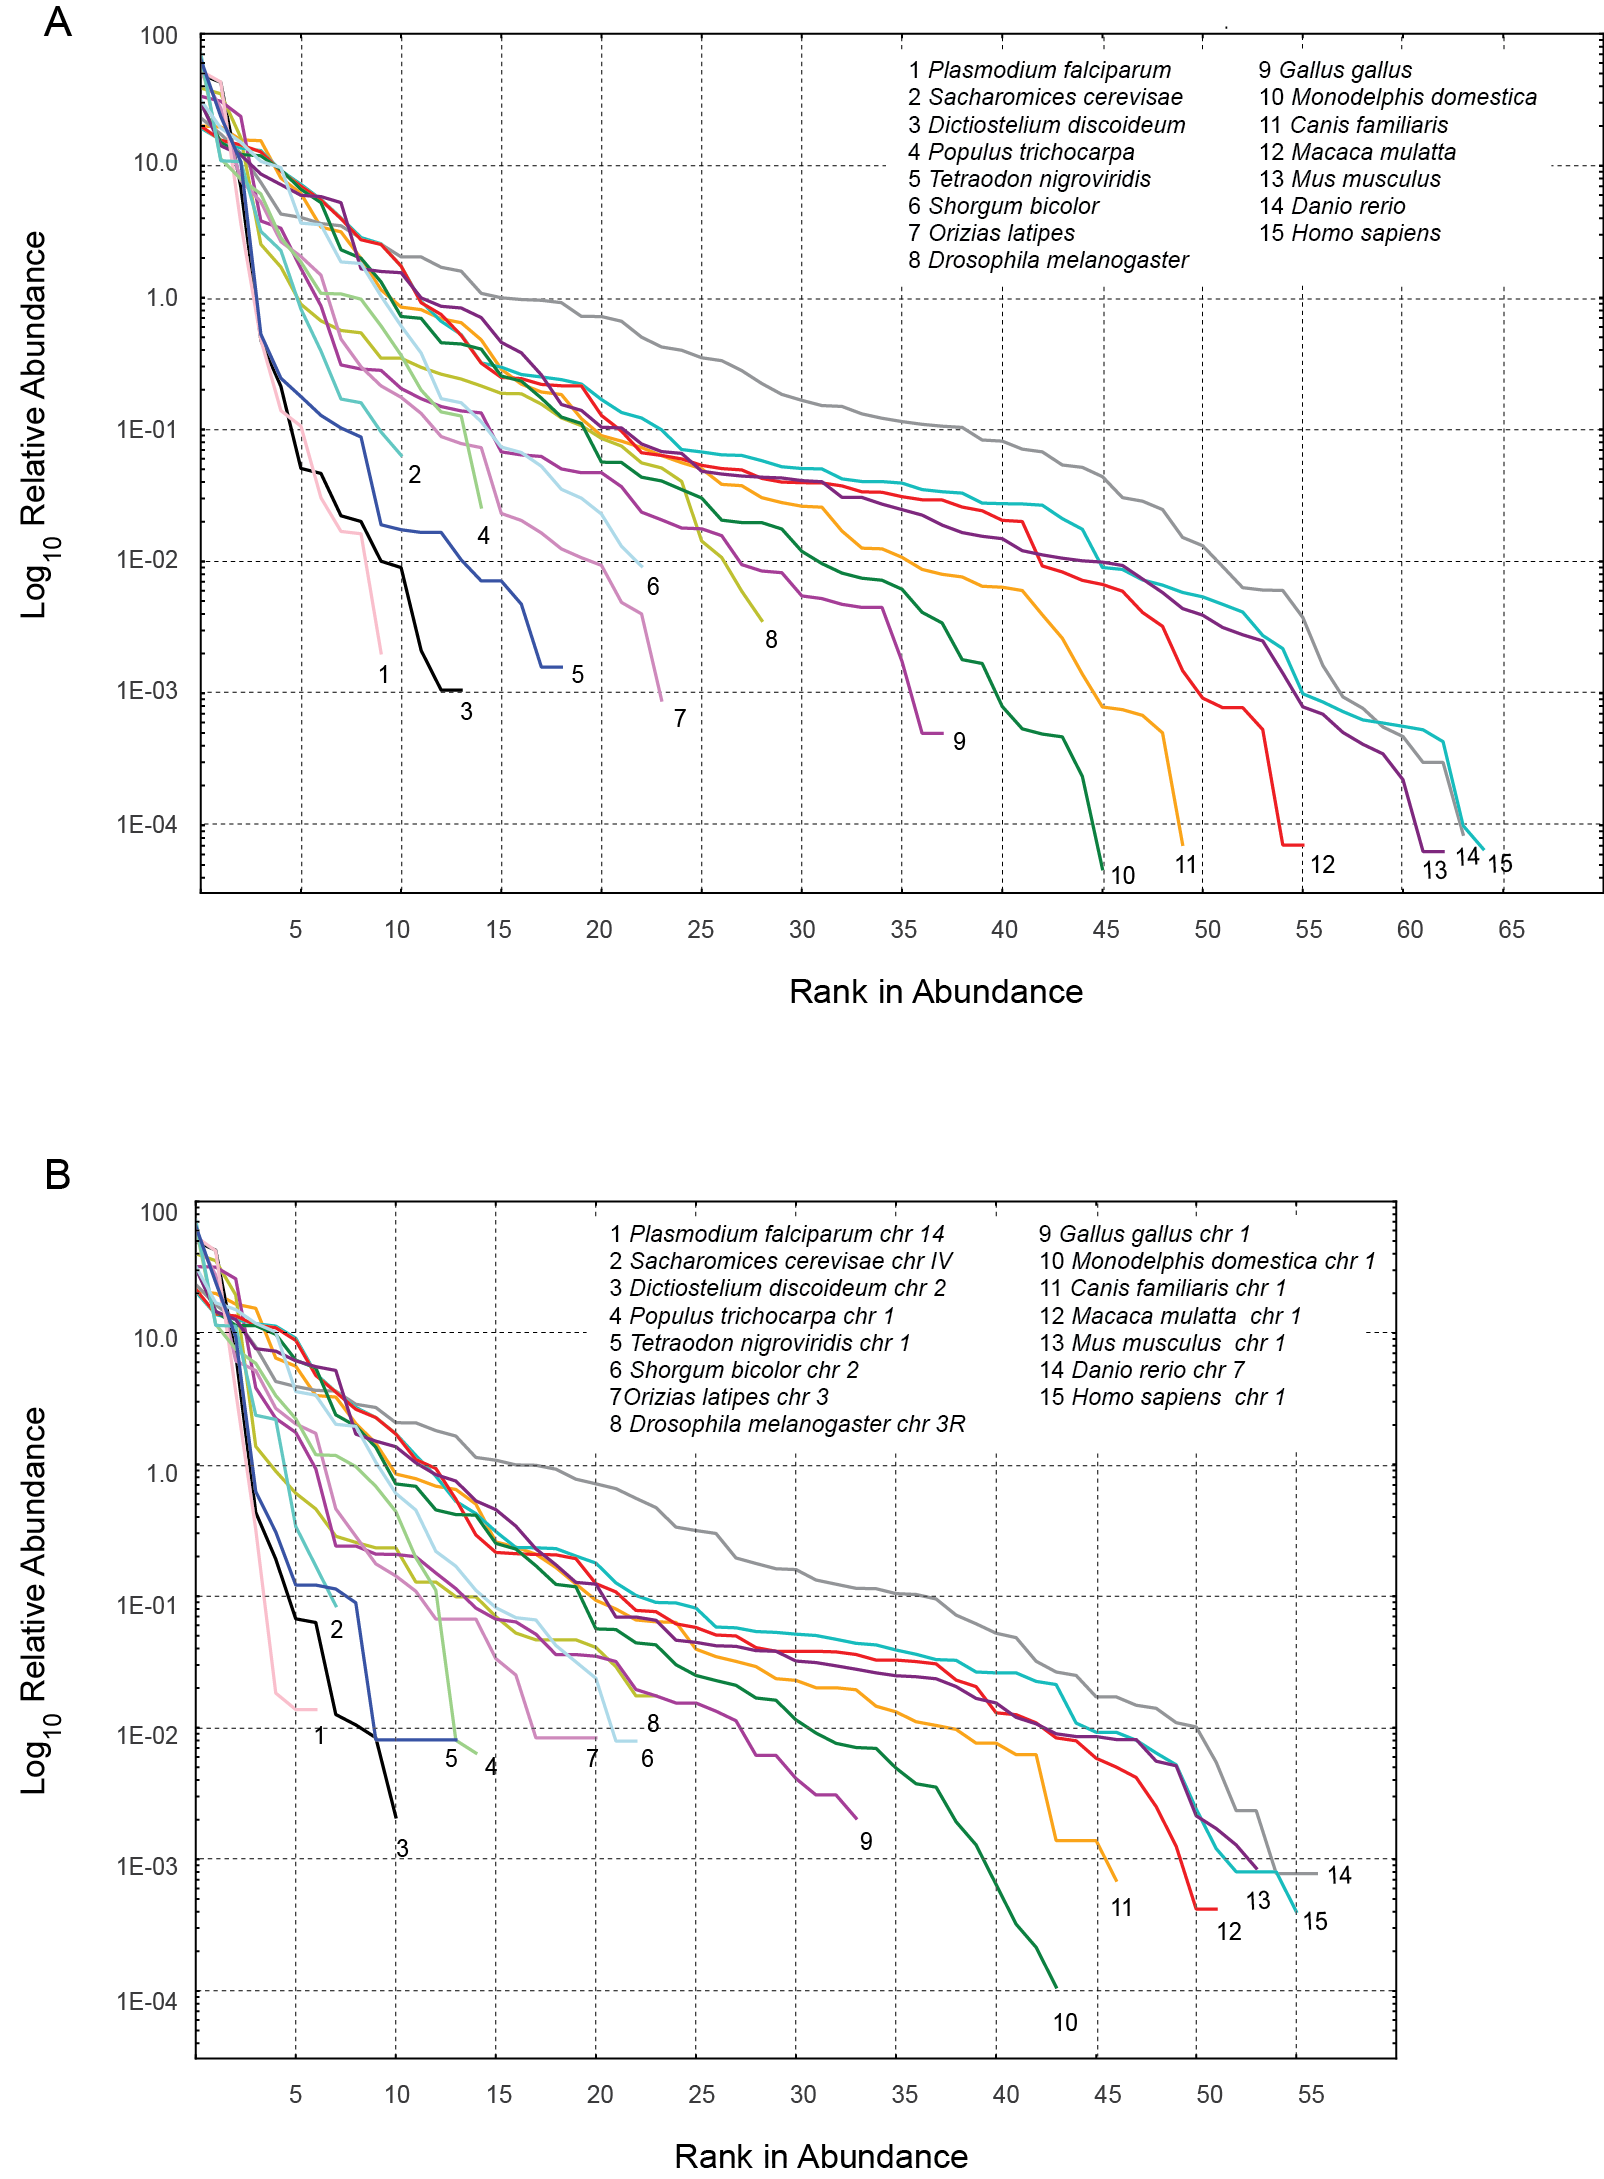
\includegraphics[width=\textwidth]{tex_source/figures/untb_genomes/SAD_genomes.png}
\caption[RSA curves.]{{\bf RSA curves.} \\ Relative species abundances for some selected genomes (A) and their corresponding largest chromosomes (B)} 
\label{fig:rsa_genomes}
\end{FPfigure}

\fref{fig:rsa_genomes}{} display RSA curves for a selected group of genomes and their largest chromosome respectively. Curves differ in many ways although two patterns are evident: 1- RSA curves of genomes and chromosomes are very similar for species, 2- all RSA curves display the universal S-shape observed in ecological environments \cite{McGill2007,Hubbell2001}. Both observations suggest a common mechanism of distribution of genetic elements in genomes and chromosomes.

\subsection{Counterbalanced species abundances in genomes}

To what extent chromosome's RSA curves represent the random distribution of the complete set of elements of the genome? To answer, we simulate the random distribution of the full set of genetic elements reported in genomes in their corresponding chromosomes. After one thousand simulations the mean expected abundance and its standard deviation were computed for all genetic classes in chromosomes. These values were used to plot random expected RSA curves for chromosomes.

Statistical tests (t-test, $FDR<0.05$) established that less than 1\% of all genetic classes in all chromosomes tested showed abundances according to their random expected distribution. This homogeneous process therefore, does not account for the observed RSA curves in chromosomes. However, another kind of arbitrary process is suggested for chromosomes if simulated and observed RSA curves are superimposed \fref{fig:rsa_chromosomes}{}.

\begin{FPfigure}
\centering 
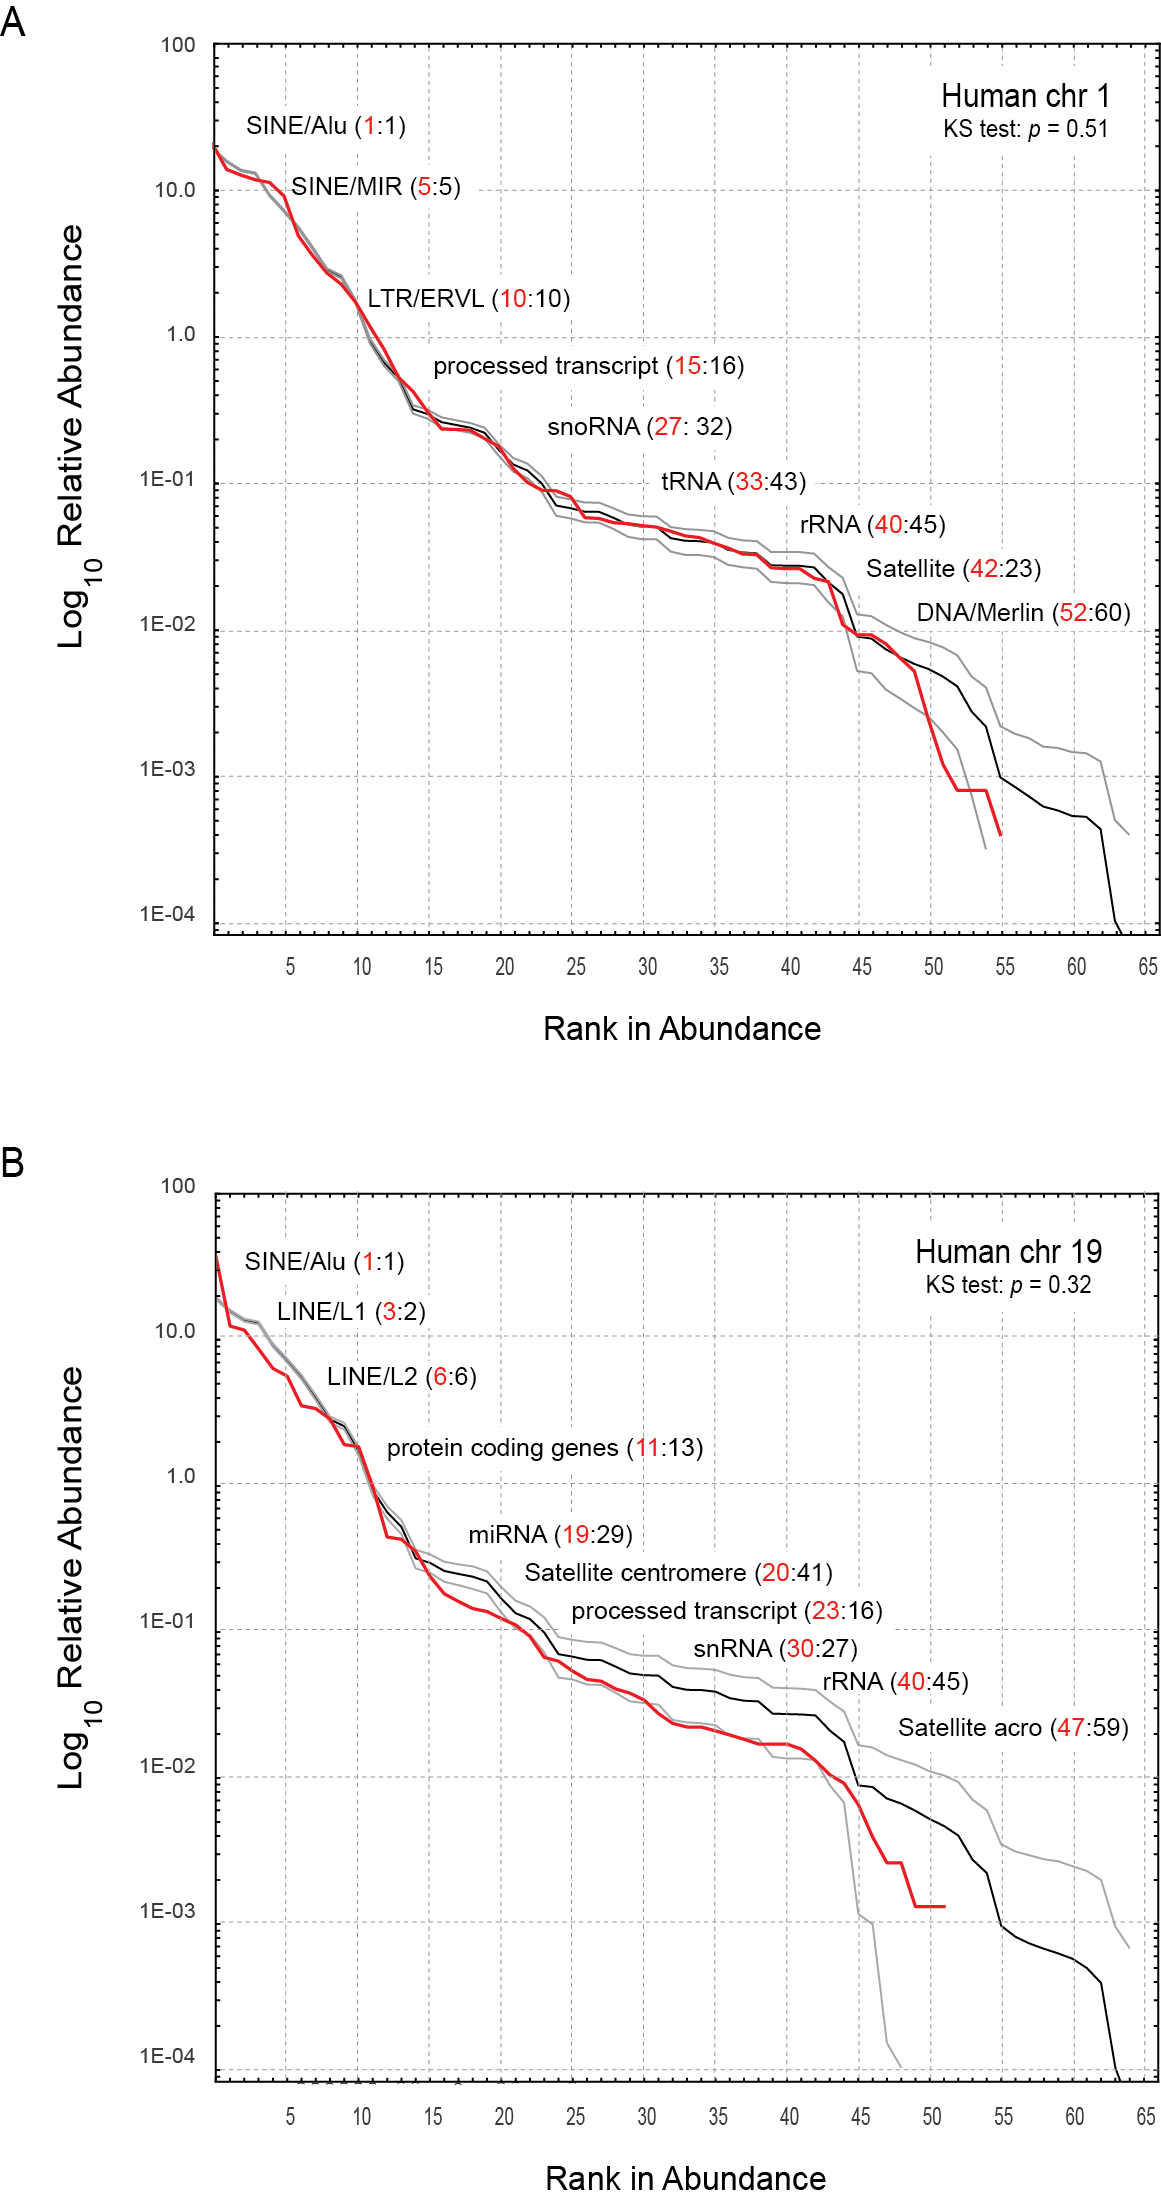
\includegraphics[height=\textheight]{tex_source/figures/untb_genomes/ra_chroms.png}
\caption[Relative species abundance curves for human chr 1 and chr 19]{{\bf Relative species abundance curves for human chr 1 (A) and chr 19 (B).} \\ Relative species abundance curves for human chr 1 (A) and chr 19 (B). Red and black lines display observed and simulated RSA curves for all functional and non-functional genetic classes in chromosomes respectively. Grey lines show two standard deviations around the mean of the simulated data. The absence of statistical differences between RSA curves is mainly due to the frequent counterbalanced changes observed in the ranking of abundances of genetic classes. Numbers in parenthesis depict the observed (red) and the expected value (black) in the ranking of abundances for few genetic classes in both chromosomes. Differences between numbers point out over and under abundances in chromosomes. Note the higher than the expected number of SINE/Alu elements in human chromosome 19 (class 1 in the ranking).} 
\label{fig:rsa_chromosomes}
\end{FPfigure}

This notable adjustment is due to the fact that genetic classes are unlabeled in the ranking order, and changes in the order of abundances are counterbalanced in chromosomes. For instance, the classes of functional tRNA and satellite elements are at position 33 and 42 of the ranking of abundances respectively in human chromosome 1 \fref{fig:rsa_chromosomes}{-A}. However, according to their random distribution the expected values in the ranking are 43 and 23 respectively. That is, tRNA and satellite elements show higher and lower abundances than the expected by random distribution. Over and under abundances of different genetic classes counterbalance each other in the same chromosome leading to an almost perfect fit between observed and expected RSA curves. We only found significant differences between observed and expected RSA curves for less than 100 of most 540 chromosomes tested (KS test, $p < 0.05$).

What is the mechanism contributing to this counterbalanced dynamics of genetic elements in eukaryote's chromosomes? Next, we test the neutral theory of biodiversity as the main explanation accounting for such events in genomes.


\subsection{Neutrality of SAD}

Similar to the kinetic theory of ideal gases in physics the neutral theory of biodiversity is a stochastic theory assuming equivalence among interacting individuals. The theory assumes that diversity in a local community of individuals is maintained by migration from the metacommunity at a constant rate ($m$). Births and deaths in the local community occur at constant rates during generation regardless the species. The metacommunity dynamics is controlled by speciation at a single constant rate ($\nu$)\cite{Rosindell2011,Alonso2006}.

For genomes, we realized that each chromosome is the physical arena where genetic elements die and are replaced by other elements of the same or different species. These genetic elements could come from the same chromosome, or from any other chromosome of the genome. We assume that each chromosome represents a local community of $J$ elements and $S$ different genetic classes (species) while the rest of chromosomes correspond to the metacommunity of size $J_M$. Thus, given the total number of functional and non-functional elements in each chromosome we optimized by maximum likelihood (ML) the neutral theory's parameters m and $\theta$ ($= 2 J_M\nu$) using Ewens and Etienne's sampling formulas (see example \fref{fig:lnl_chrom}{}).

Deviations of neutrality were detected in 33 out of 578 (5.7\%) chromosomes. However, deviations vanished at all after multiple testing correction ($FDR< 0.05$, Table). We conclude that Hubbell's neutral model fits abundance and diversity of genetic elements in all the chromosomes of the 31 eukaryotes genomes analyzed. 


\subsection{Diversity and chromosome length}

\section{Discussion}

Abundance and diversity of selfish genetic elements \cite{Doolittle1980,Orgel1980} results from millions of years of close interaction with their host, the genome. Population dynamics models dealing with transposable elements (TE) has been formalized and reviewed \cite{Charlesworth2009,Charlesworth1994,LeRouzic2005}. Transposition and excision rates, as well as host fitness impact are some of their most significant parameters. While the predicted deleterious effects of transposition have been confirmed repeatedly in Drosophila (citar...), almost a neutral accumulation of TEs is expected in mammals due to the larger genomes and smaller population size18. An important concern with these models is the explicit absence of relationships of TEs with other genetic components of the genome. 

The general transposition-selection based model predicts an adaptive equilibrium of TE abundance. However, abundances of the same TE differ between population and species (citar). 
Additionally, models c 9-11. Importantly variation between individuals was observed...\cite{Brookfield2005}

However, a former question is mandatory: Did TE's diversity and abundance features shaped by random processes in genomes \cite{Lynch2003,Venner2009}. 

Nature seems to play forest and genomes with the same dice.
Functional elements, as expected deviates expectations If functional elements are excluded from chromosomes, neutrality was rejected in a single chromosome (D. rerio chr2, p= 0.04, q= 0.36).


\section{Material Methods}

\subsection{Genomes}

31 genomic sequences were used, all re-used from previous work see Section \ref{sec:complexity-strings}.

\subsection{Mining of Genomic Elements}

RepeatMasker.

\subsection{Ecolopy}

\subsubsection{Ecological models}

\paragraph{Ewens}

\paragraph{Etienne}

\paragraph{Log-Normal}

\subsection{Model optimization}
\label{sec:model-optimization}

Models where optimized through different optimization strategies depending on the model selected. In the case of the Ewens' formula, $\theta$ is the only parameter to take into account, and its estimation is achieved with the \textit{golden} optimization strategy \cite{Jones2001}. For Etienne's model, two parameters were optimized, $\theta$ and $m$, using the best solution of the \textit{downhill simplex algorithm} \cite{Nelder1965}, \textit{L-BFGS-B algorithm} \cite{Byrd1995}, \textit{truncated Newton algorithm} \cite{Nash1984} and \textit{Sequential Least SQuares Programming} all implemented in \textit{Scipy} \cite{Jones2001}.

Optimization step being critical specially under Etienne model, the likelihood surface of the model given a value of $\theta$ and $m$ was drawn for some of the chromosomes in our dataset. This procedure allows us to find  graphically the best solution for both parameters. The solution found by this methodology was then compared to the optimization result, in order to validate them (see \fref{fig:lnl_chrom}{} as an example of this validation step).

\begin{figure}[htpb]
\centering 
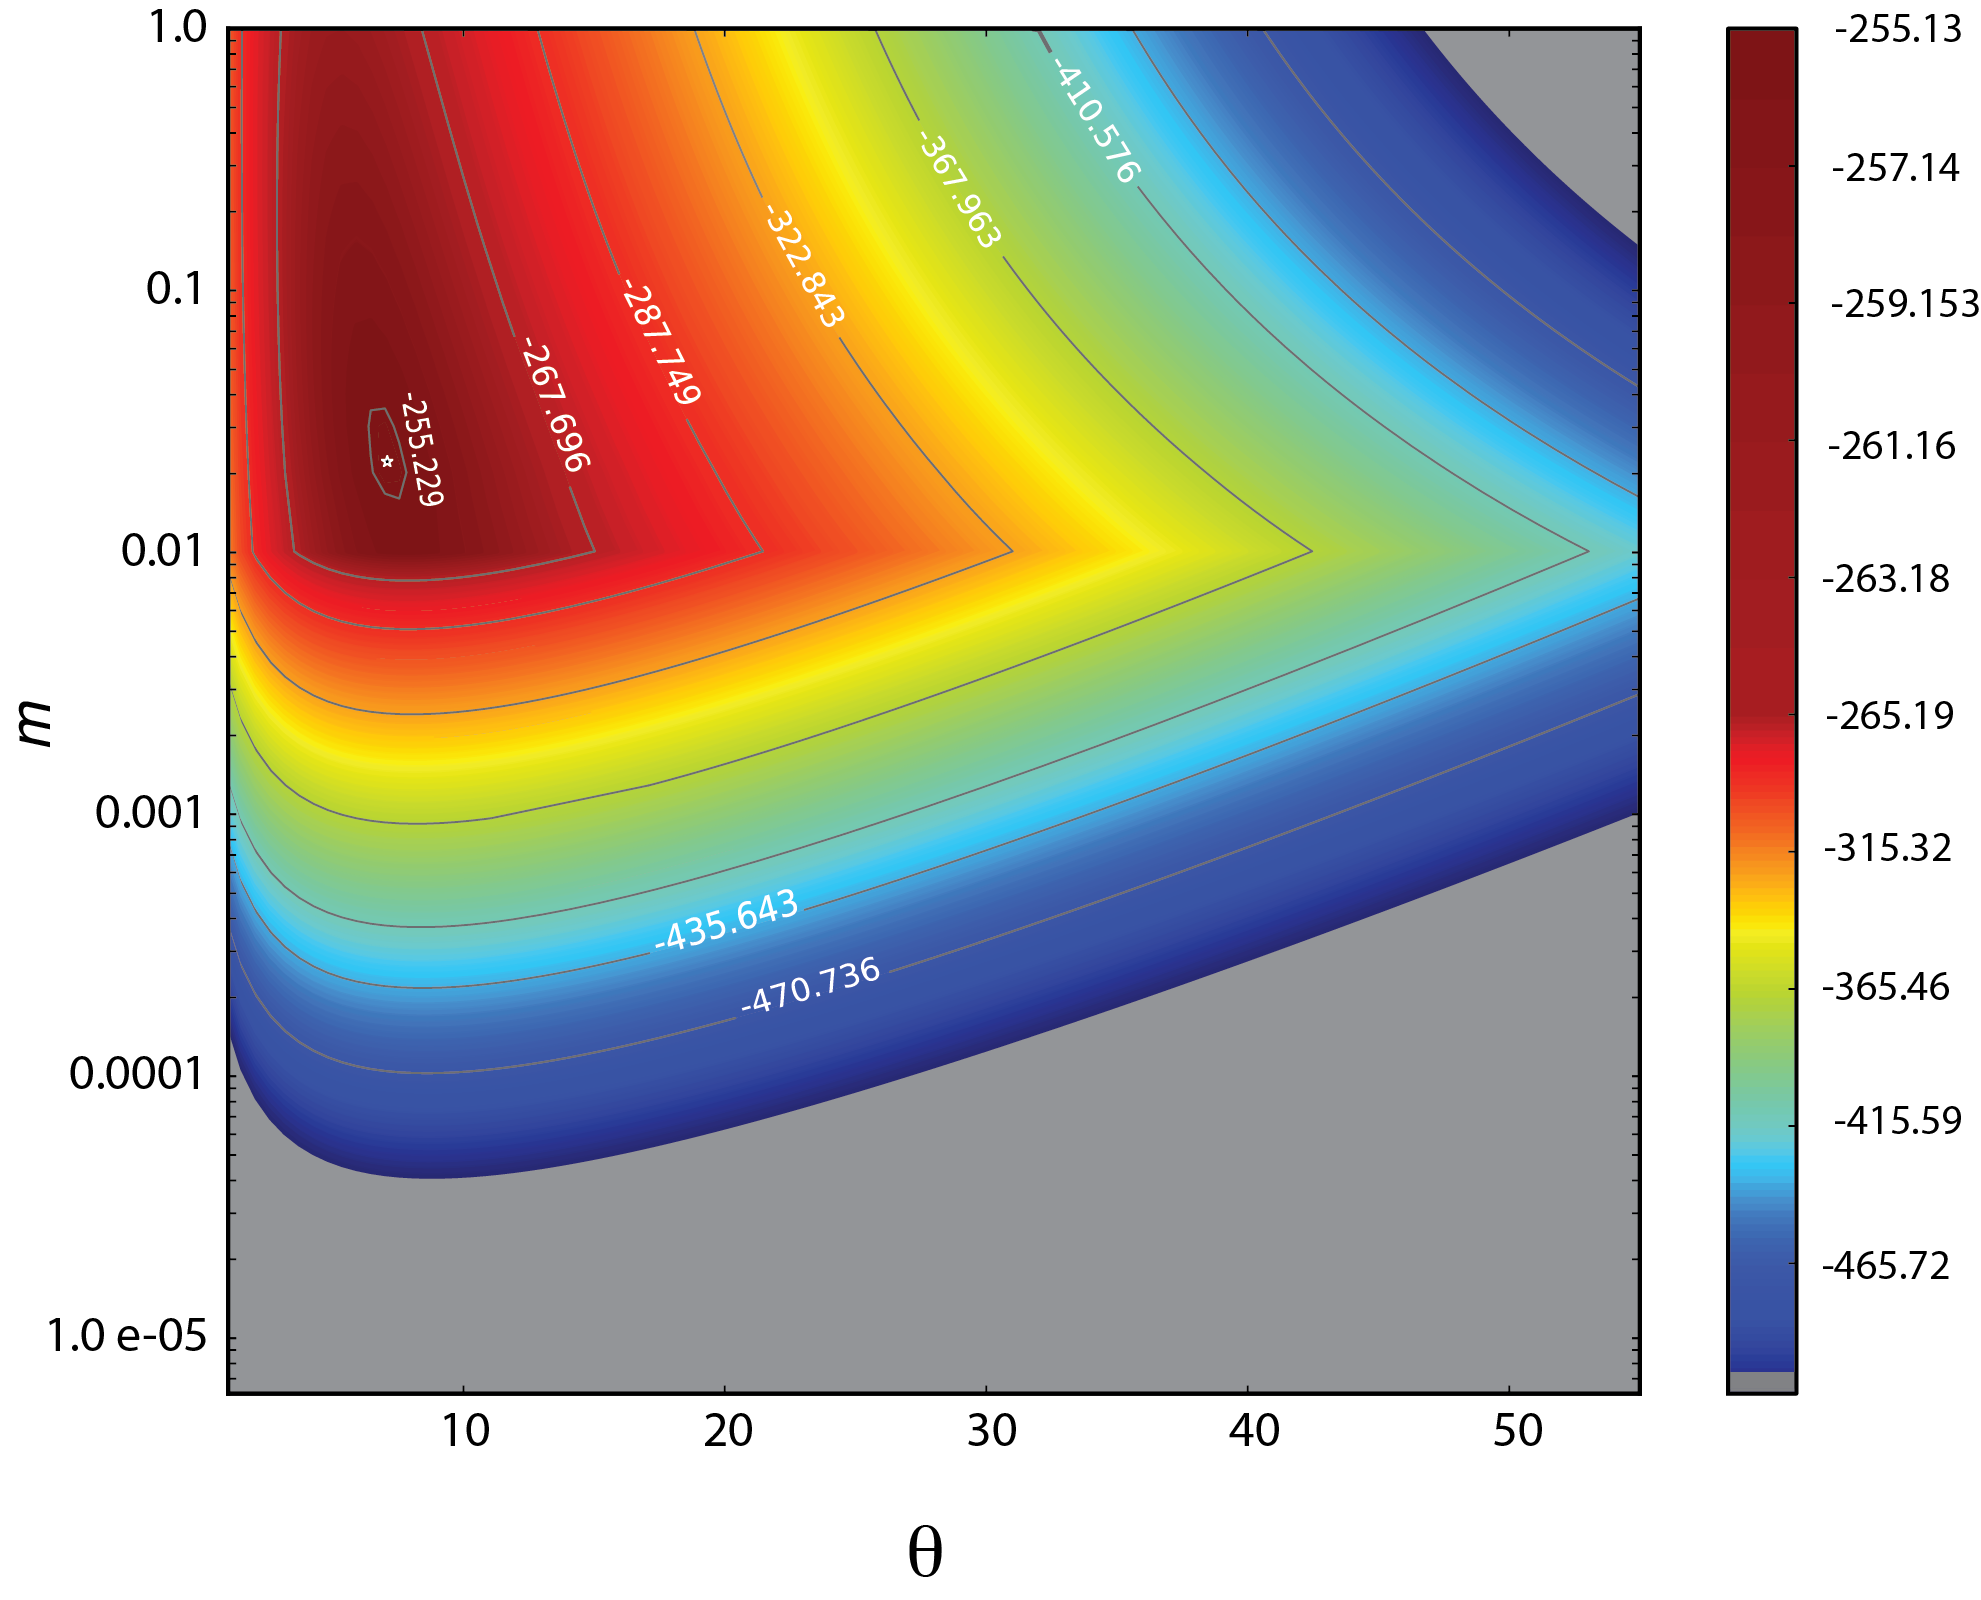
\includegraphics[width=\textwidth]{tex_source/figures/untb_genomes/lnl_chrom.png}
\caption[Maximum likelihood inference of neutral parameters.]{{\bf Maximum likelihood inference of neutral parameters.}\\ Log likelihood surface as a function of migration rate ($m$), and the fundamental biodiversity number ($\theta$) for \textit{D. rerio} chromosome 19. Dark red color shows regions of the surface where parameters maximize the probability to explain abundances and diversity of genetic elements in the chromosome. Likelihood ratio tests favored Etienne in contrast to Ewens sampling formula to explain the observed data in the chromosome.}
\label{fig:lnl_chrom}
\end{figure}

\subsection{Model testing}

In order to compare and test the fit of the two models computed, a likelihood ratio test \cite{Wilks1938} was conducted thanks to the fact that Etienne's model is nested into Ewens'. Etienne's model has two free parameters while Ewens' only one (under this model $m$ parameter is fixed to 1), thus the number of degrees of freedom for the chi-squared distribution is 1.

Additionally, given the large number of test performed, statistical significances were corrected by false discovery rate (FDR) \cite{Benjamini2001}. Etienne's model was thus kept as best fit model for only those chromosomes that pass the LRT after FDR adjustment, otherwise the null model using Ewens' formula was selected.

\subsection{Test for neutrality}

In the last years two exact tests were developed in order to accept or reject the neutrality of a given community. Both tests are based on the comparison of a given number of random neutral community generated using the parameters estimated (see \ref{sec:model-optimization}) for the real data under neutrality. The comparison of the random neutral communities with the observed distribution of abundances, is the key point to test for neutrality.

The first of these tests \cite{Etienne2007} consists in comparing the distribution of likelihoods of fitting neutral model. This corresponding distribution of random neutral abundances is compared to the likelihood of the observed data. The major problem of this test is technical, the computation time needed to optimize the parameters of each abundance distribution and get the likelihoods is unrealistically too high when dealing with genomic elements.

The second test \cite{Jabot2011} uses, instead of likelihood, the comparison of Shannon's entropy, and is much faster as random neutral abundances do not need to be fitted into a neutral model.

Thus, from the neutral parameters obtained for each chromosome, we simulated distribution of abundances of genetic elements 10,000 times. 

To test for the UNTB the evenness of each simulated distribution was computed using the Shannon's entropy H \cite{Jabot2011}. The set of H values conform the neutral null distribution to test if the empirical H of chromosomes is beyond the expected by random \fref{fig:shannon_distrib}{}.


\begin{figure}[htpb]
\centering 
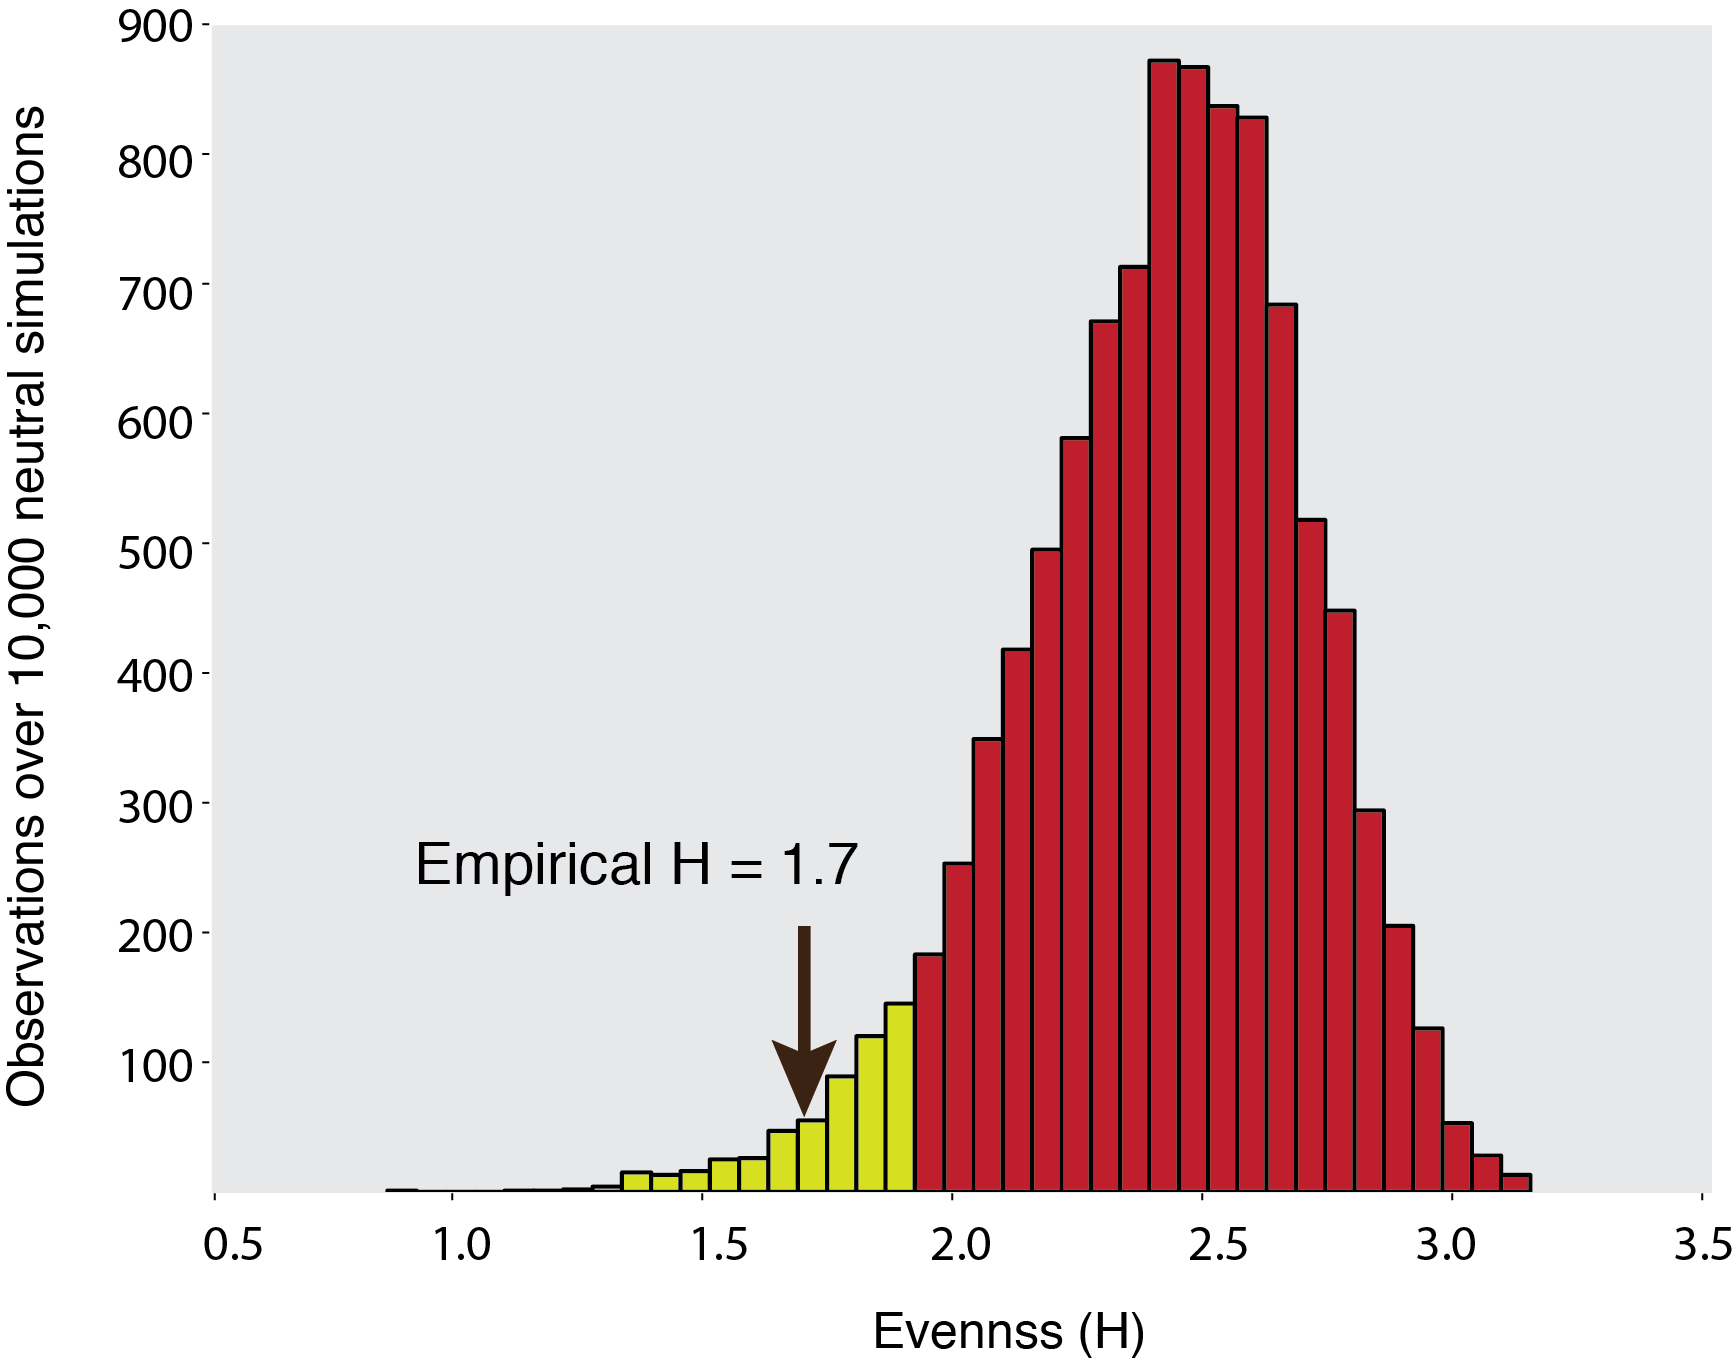
\includegraphics[width=\textwidth]{tex_source/figures/untb_genomes/shannon_distrib.png}
\caption[Comparing simulated and empirical evenness.]{{\bf Comparing simulated and empirical evenness. }\\Neutrality test statistically compares simulated null distribution of H with the empirical H value of the corresponding chromosome. In this case, the null distribution of H values was derived from 10,000 neutral simulations of A. gambiae chromosome 2L, with neutral parameters ($\theta$ and $m$) optimized by ML using Etienne sampling formulae. Yellow and red bars display 5\% and 95\% of the simulated neutral data, respectively. Although in this case neutrality was rejected (p= 0.01), posterior correction by multiple testing favored the null neutral hypothesis (q= 0.21).}
\label{fig:shannon_distrib}
\end{figure}



%%% Local Variables: 
%%% mode: latex
%%% TeX-master: "../../master"
%%% End: 
